\documentclass{article}
\usepackage{graphicx}
\usepackage{parskip}
\usepackage{listings}
\usepackage{syntax}
\author{Alexander Wood}
\title{Computer Science Notes}
\begin{document}

\maketitle
  
\tableofcontents


\section{Regular Expressions}
Regular Expressions can be used to validate emails, password, or variables 
and functions in a programming language

\subsection{Control Characters}
\begin{tabular}{|l|l|l|l|l|}
\hline
* & Matches 0 or more times & \verb/ab*c/ & ab, abc, abbbbc \\ \hline
? & Matches 0 or 1 times & \verb/ab?c/ & ac, abc \\ \hline
+ & Matches 1 or more times & \verb/ab+c/ & abc, abbbbc \\ \hline
| & Matches either character & \verb/(a|b)/ & a, b \\ \hline
\end{tabular}



\subsection{BNF Notation}

Regexes can be used to validate simple syntax, but they are not suitable for complex languages.
Context-free languages are used to represent the syntax of languages with complex syntax \textbf{Backus-Naur Form (BNF)} is an example of a context-free language.
\newline
\begin{tabular}{|c|c|} 
\hline
$<$ $>$ & Encloses each element \\ \hline
::= & Defines the rule for a previous element \\ \hline
| & Used to indicate OR \\ \hline
\{ \} & Encloses optional elements \\ \hline
\end{tabular}
\newline

Each element should be broken down until a terminal element is reached. That is,
 an element that can't be broken down any further.

\begin{grammar}
<student-details> ::= <name> <address> <gender>

<address> ::= <street> <town> <county> <post-code>

<gender> ::= "M" | "F"
\end{grammar}

BNF is unambiguous, a statement can only be written in 1 way.
It can also be recursive. For example,
\begin{grammar}
<positiveInteger> ::= <nonZeroDigit>|<digit><positiveInteger>
\end{grammar}


\begin{grammar}
<digit> ::= 0 | 1 | 2 | 3 | 4 | 5 | 6 | 7 | 8 | 9

<whole-number> ::= <digit> | <digit><whole-number>

<plus-minus> ::= + | -

<integer> ::= <whole-number> | <plus-minus> <whole-number>
\end{grammar}

\subsection{Syntax Diagrams}
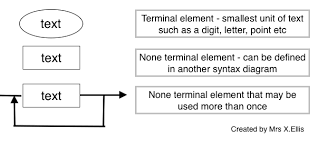
\includegraphics{syntax diagramn.png}


\end{document}